%!TEX root = these.tex

\chapter{Revue de la vérification à l'exécution et des travaux associés}

Dans ce chapitre, on revoit tout d'abord la vérification à l'exécution, y compris son histoire, sa définition et le comparaison avec d'autres techniques de vérification. D'autre part, la logique temporelle linéaire, en tant que la spécification formalisme commun de la vérification à l'exécution, est présenté avec la syntaxe, les opérateurs et la sémantique. Enfin, quelques cadres de la vérification à l'exécution bien connus sont introduits, ainsi que d'une comparaison simple d'entre eux.

\section{Vérification à l'exécution}

La vérification et la validation de logiciels, en tant qu'un aspect important de la gestion de projet et de l'ingénierie du logiciel, est le processus d'employer diverses techniques nécessaires pour détecter les violations ou les satisfactions et d'évaluer la qualité des logiciels et la performance d'un système \citep{ieeestd2012}.

\subsection{Concepts fondamentaux}

Il y a normalement deux types de techniques de vérification: analyse statique et dynamique. Certains techniques traditionnelles bien connues d'analyse statique sont la vérification de modèles \citep{clarke1999model} et la démonstration de théorèmes \citep{heisel1990tactical}. L'analyse statique est généralement appliquée pour vérifier les comportements d'un système avant son exécution, mais ces techniques ont les lacunes naturelles. Par exemple, la vérification de modèles ne peut pas fonctionner sur un système dont la taille ou le nombre d'états pourraient se développer au-delà de la capacité de puissance de calcul en raison de la ``state-explosion problem''.

L'analyse dynamique est destinée de surveiller les systèmes en cours d'exécution. Bien que parfois le résultat pourrait être faux négatifs à cause de son inachèvement, cette incomplétude permet aux techniques d'analyse dynamique de briser la limitation de méthodes statiques et devenir ainsi les méthodes complémentaires de la vérification. \citep{falcone2013tutorial}

La vérification à l'exécution est une sorte de technique de vérification sur la base de l'analyse dynamique. En 2001, le Runtime Verification workshop\footnote{http://www.runtime-verification.org/} a été fondée, comme la terminologie ``runtime verification'' était officiellement introduite \citep{wiki:rv}. Elle est une technique relativement nouvelle qui est légère et qui vise à compléter d'autres techniques traditionnelles de vérification comme ``model checking'' et ``testing''.

\cite{leucker2009brief} définissent la vérification à l'exécution comme suit:

\begin{displayquote}
Runtime verification is the discipline of computer science that deals with the study, development, and application of those verification techniques that allow checking whether a run of a system under scrutiny satisfies or violates a given correctness property.
\end{displayquote}

Normalement, lorsqu'une violation est observée, la vérification à l'exécution ne résout pas le programme détecté elle-même, mais son résultat est un guide et base importante pour d'autre composants dans le même système pour régler le problème.

\cite{leucker2009brief} définissent également un \emph{run} d'un système en tant qu'une séquence de traces infinies du système, et une \emph{exécution} d'un système comme une trace finie et aussi un \emph{préfixe fini} de un \emph{run}. Le travail de vérification à l'exécution se concentre principalement sur l'analyse de \emph{exécutions} qui sont effectuées par les \emph{moniteurs}.

Un \emph{moniteur} est une procédure de décision générée (ou ``synthétisée'') à partie de l'une des propriétés formelles qui doit être vérifiée contre l'exécution du système donné. Lors de la vérification, un \emph{moniteur} énumère les traces finies d'un \emph{exécution}, vérifie si elles satisfont aux propriétés d'exactitude et produit un \emph{verdict} comme le résultat. Un \emph{verdict}, qui est normalement une valeur de vérité, indique la satisfaction de la propriété contre les événements recueillis.

Un verdict dans la plupart des cas simples peut être normalement exprimée comme vrai/faux, oui / non ou 1/0, selon le contexte. Mais en réalité, de nombreux systèmes de la vérification à l'exécution doivent introduire d'autres valeurs pour fournir un résultat plus précis. Par exemple, grâce à l'incomplétude du système de la vérification à l'exécution, un verdict ne peut pas être facilement émis lorsque le moniteur a besoin de plus d'événements successifs, donc une valeur \emph{inconcluante} (écrite comme ``?'') est introduite pour indiquer l'état présent du système surveillé. \citep{falcone2013tutorial}

\subsection{Procédure}

\begin{figure}[h]
\begin{center}
\centering
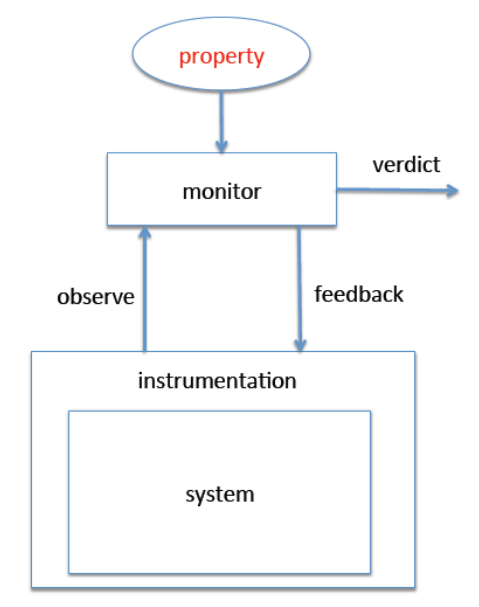
\includegraphics[width=80mm]{rvstruct.png}
\caption{Processus de la vérification à l'exécution (de \cite{falcone2013tutorial})}
\label{img:rvstruct}
\end{center}
\end{figure}

La figure \ref{img:rvstruct} décrit le processus d'un système typique de la vérification à l'exécution qui contient quatre étapes suivantes \citep{falcone2013tutorial}:
\begin{enumerate}
\item \emph{Synthèse du moniteur}: Un moniteur est synthétisé à partir d'une propriété.
\item \emph{Instrumentation du système}: Les instruments supplémentaires sont intégrés au système sous surveillance afin de générer les événements pour le \emph{moniteur}.
\item \emph{Exécution}: Le système est exécuté et commence à générer les événements et les envoie au moniteur.
\item \emph{Analyse et réponse}: Le moniteur analyse les événements collectés, émet un \emph{verdict} et envoie les informations supplémentaires, disons les \emph{commentaires}, au système si nécessaire.
\end{enumerate}

Les moniteurs peuvent être classés en plusieurs modes d'aspects différents \citep{chen2007mop}:
\begin{itemize}
\item \emph{online/offline} dépend du moment où les moniteurs et le système fonctionnent: \emph{Online} s'ils travaillent en même temps, et \emph{offline} si les moniteurs commencent à travailler après la fin de l'exécution du système.
\item \emph{inline/outline} dépend de l'endroit où les moniteurs sont exécutés: \emph{Inline} si les moniteurs sont embarqués dans le système et \emph{outline} si les moniteurs fonctionnent tout seuls en recevant les traces d'événements du système par certaines méthodes, par exemple par un système de fichiers ou par un signal sans fil.
\item \emph{violation/validation} est déterminé par la spécification du verdict.
\end{itemize}

D'après les définitions des modes, on peut apercevoir qu'un moniteur travaillant en mode \emph{offline} travaille également en mode \emph{outline} et le mode \emph{inline} implique le mode \emph{online}.

\subsection{Comparaison avec d'autres techniques}

Comparant avec la vérification de modèle \citep{clarke1999model} qui vise à vérifier les systèmes d'états finis, on voit que les méthodes de génération de moniteurs dans la vérification à l'exécution et de la génération d'automates dans la vérification de modèle ont des similitudes. Cependant, alors que la vérification de modèle traite principalement les traces infinies, la vérification à l'exécution ne traite que les traces finies, i.e. les \emph{exécutions}. Pour cette raison, les moniteurs de la vérification à l'exécution travaillant en mode \emph{online} doivent être en mesure d'accepter les traces supplémentaires.

Une autre différence importante entre la vérification de modèle et la vérification à l'exécution est que, contrairement à la vérification de modèle qui vérifie si toutes les \emph{exécutions} d'un système satisfont une propriété d'exactitude, la vérification à l'exécution est intéressée uniquement par le fait qu'il y a ou non une \emph{exécution} qui appartient à un ensemble d'exécutions valides. En outre, la vérification à l'exécution ne nécessite qu'analyser les événements observés d'un système donné, sans avoir à regarder ses informations intérieures, mais dans la vérification de modèle, le modèle correct du système doit être reconnu afin de préparer chaque exécution possible avant de l'exécution du le système. \citep{leucker2009brief}

Le test du logiciel \citep{broy2005model} est une autre technique de vérification. Elle est un processus de l'exécution d'un programme avec un ensemble fini de séquences entrée-sortie qui est nommé ``la suite de tests''. Comparant avec la vérification à l'exécution, les suites de test sont définies directement, à la différence des propriétés de la vérification à l'exécution qui sont générées à partir des spécifications de formalisme. En outre, ``le test exhaustif'' qui est une méthode courante dans le test du logiciel, n'est normalement pas une option de la vérification à l'exécution.

\section{Logique Temporelle Linéaire}

Dans la vérification à l'exécution, un moniteur est traduit à partir d'une propriété d'exactitude, et les propriétés d'exactitude sont spécifiés dans les logiques temporelles en temps linéaire, telles que la logique temporelle linéaire.

La logique temporelle est une extension de la logique classique, et elle fournit un langage pratique avec les expressions des propriétés pour raisonner sur le changement des états en termes de temps. Bien qu'il y ait beaucoup de logiques temporelles différentes qui sont inventées pour satisfaire aux exigences diverses, les logiques temporelles sont normalement classées par le fait que le temps est linéaire ou en ramification. La logique temporelle avec le temps linéaire est appelé \emph{Logique Temporelle Linéaire} (LTL), qui a d'abord été proposé par \cite{pnueli97}. le temps dans la LTL est transformé en une séquence d'états qui s'étendent vers le futur infini. La séquence d'états est un \emph{chemin} de calcul. \citep{clarke1999model} \cite{huth2004}

\cite{leucker2009brief} résument la LTL comme une logique temporelle en temps linéaire qui est bien acceptée et utilisée pour spécifier les propriétés de traces infinies. Néanmoins, dans la vérification à l'exécution, la LTL est employée pour vérifier les exécutions finies.

\subsection{Syntaxe}

Une formule bien formée de la LTL consiste en un ensemble fini de propositions atomiques, des opérateurs booléens $\neg, \wedge, \vee, \rightarrow$ et des opérateurs de logiques temporelles \textbf{F}(future), \textbf{G}(global), \textbf{X}(next), \textbf{U}(until), \textbf{W}(weak-until) et \textbf{R}(release). Elle peut être représenté sous la forme Backus Naur comme suit \citep{huth2004}:
\begin{align}
\phi ::= & \top | \bot | p | (\neg\phi) | (\phi \wedge \phi) | (\phi \vee \phi) | (\phi \rightarrow \phi) \nonumber \\
& | (\X \phi) | (\F \phi) | (\G \phi) | (\phi \U \phi) | (\phi \W \phi) | (\phi \R \phi)
\end{align}

\subsection{Sémantiques}

Pour une séquence d'états $s_0, s_1, s_2, ..., s_i, s_{i + 1}, ... $ où $s_{i + 1}$ est un état futur de $s_i$, on définit un chemin avec $\pi^i = s_i \rightarrow s_{i + 1} \rightarrow ... $ où $i$ est le premier état dans ce chemin. Étant donné que $\pi(i)$ est l'ensemble de propositions atomiques qui sont vraies au $i$ème état, le fait qu'un chemin $\pi^i$ satisfait ou non une formule de la LTL est définie comme suit \citep{rozier2011linear}:

\begin{itemize}
  \item \listequation{\pi^i \vDash \top} \label{eq:true}
  \item \listequation{\pi^i \nvDash \bot} \label{eq:false}
  \item \listequation{\pi^i \vDash p \iff p \in \pi(i)} \label{eq:ap}
  \item \listequation{\pi^i \vDash \neg\psi \iff \pi^i \nvDash \psi} \label{eq:not}
  \item \listequation{\pi^i \vDash \psi \wedge \varphi \iff \pi^i \vDash \psi \text{ et } \pi^i \vDash \varphi} \label{eq:and}
  \item \listequation{\pi^i \vDash \psi \vee \varphi \iff \pi^i \vDash \psi \text{ ou } \pi^i \vDash \varphi} \label{eq:or}
  \item \listequation{\pi^i \vDash \psi \rightarrow \varphi \iff \pi^i \vDash \varphi \text{ chaque fois que } \pi^i \vDash \psi} \label{eq:then}
  \item \listequation{\pi^i \vDash \X \psi \iff \pi^{i + 1} \vDash \psi} \label{eq:next}
  \item \listequation{\pi^i \vDash \G \psi \iff \forall j \geq i, \pi^j \vDash \psi} \label{eq:global}
  \item \listequation{\pi^i \vDash \F \psi \iff \exists j \geq i, \pi^j \vDash \psi} \label{eq:future}
  \item \listequation{\pi^i \vDash \psi \U \varphi \iff \exists j \geq i, \pi^j \vDash \varphi$ et $\forall k, i \leq k < j, \pi^k \vDash \psi} \label{eq:until}
  \item \listequation{\pi^i \vDash \psi \W \varphi \iff$ soit $\exists j \geq i, \pi^j \vDash \varphi$ et $\forall k, i \leq k < j, \pi^k \vDash \psi$, $ \\ $soit $\forall k \geq i, \pi^k \vDash \psi} \label{eq:wuntil}
  \item \listequation{\pi^i \vDash \psi \R \varphi \iff$ soit $\exists j \geq i, \pi^j \vDash \psi$ et $\forall k, i \leq k \leq j, \pi^k \vDash \varphi$, $ \\ $soit $\forall k \geq i, \pi^k \vDash \varphi} \label{eq:release}
\end{itemize}

Les formules \ref{eq:true} et \ref{eq:false} suggèrent que les états dans le chemin $\pi^i$ devraient toujours être vrais ou faux.

Dans la formule \ref{eq:ap}, $p$ est une proposition atomique appartenant à l'ensemble fini de propositions atomiques de la LTL, et cette formule demande de vérifier seulement le $i$ème état.

Les formules \ref{eq:not}---\ref{eq:then} sont les opérateurs booléens de la logique propositionnelle qui respectent les règles du tableau \ref{table:prologic}.

\begin{table}[h]
\centering
\begin{tabular}{|c|c|c|c|c|c|}
\hline
$\psi$ & $\varphi$ & $\neg\psi$ & $\psi \wedge \varphi$ & $\psi \vee \varphi$ & $\psi \rightarrow \varphi$ \\
\hline
Vrai & Vrai & Faux & Vrai & Vrai & Vrai \\
\hline
Vrai & Faux & Faux & Faux & Vrai & Faux \\
\hline
Faux & Vrai & Vrai & Faux & Vrai & Vrai \\
\hline
Faux & Faux & Vrai & Faux & Faux & Vrai \\
\hline
\end{tabular}
\caption{La table de vérité des opérateurs booléens de la logique propositionnelle}
\label{table:prologic}
\end{table}

Les formules \ref{eq:next}, \ref{eq:future} et \ref{eq:global} sont les conjonctions unaires de logiques temporelles . L'opérateur\X signifie ``la prochaine fois'' et il saute le $i$ème état et évalue le chemin $\pi^{i + 1}$. L'opérateur\F signifie ``parfois dans l'avenir'' qui exige que dès le $i$ème état, une propriété reste valide dans un état futur sur le chemin. Et l'opérateur\G (``globalement'' ou ``toujours'') indique qu'une propriété devrait reste valide dans chaque état depuis la $i$ème état jusqu'à la fin ou le futur infini.

Les formules \ref{eq:until}, \ref{eq:wuntil} et \ref{eq:release} sont les opérateurs binaires de logiques temporelles. L'opérateur\U est l'abréviation de ``until''. La formule $\psi \U \varphi$ reste valide si $\varphi$ reste valide à un état futur sur le chemin, et avant cet état, la propriété $\psi$ reste valide à chaque état. L'opérateur\W est une version faible de l'opérateur\U, sauf que pour la formule $\psi \W \varphi$, $\varphi$ n'a pas besoin de rester valide à terme dans un état futur. L'opérateur\R, qui signifie ``libérer'', est en fait une logique duale de l'opérateur\U, i.e. $\psi \U \varphi \equiv \neg (\neg \psi \R \neg \varphi)$. L'opérateur\R exige que pour la formule $\psi \R \varphi$, la propriété $\varphi$ devrait continuellement rester valide jusqu'à $\psi$ devient valide et $\psi$ n'a pas besoin de rester valide à terme.

Il convient de noter que dans la LTL, les logiques à deux valeurs pourraient donner un résultat prématuré qui est vrai ou faux. Tel que mentionné précédemment, la LTL est définie pour travailler avec les traces infinies tandis que le monitoring de la vérification à l'exécution est seulement capable de traiter les traces finies, ce qui pourrait conduire à un conflit, en particulier dans un système en cours d'exécution. Par exemple, $\F \psi$ indique que $\psi$ devraient rester valide dans un état futur. Dans un système actif, tant que $\psi$ ne reste pas valide dans les états observés, les résultats de la formule sont toujours $faux$, mais si $\psi$ devient valide dans l'observation suivante, les résultats précédents deviendra corrompus et obsolètes. Par conséquent, \cite{bauer2006monitoring} ont proposé la logique à trois valeurs (LTL$_3$) qui introduit une nouvelle valeur \emph{inconcluant} pour les cas où la propriété ne peut pas être évaluée immédiatement.

\subsection{Diverses logiques temporelles}

\subsubsection{Metric Temporal Logic}

Metric Temporal Logic (MTL) \citep{chang1994compositional} a été inventé pour raisonner sur les propriétés en temps réel. Pour préciser le temps avec précision, MTL coupe le temps en morceaux numérotés qui sont également appelés les modules de transition chronométrés, et emploie les opérateurs aux limites pour contraindre les opérateurs de logiques temporelles. Ses formules sont définies comme suit:
\begin{align*}
\phi ::= & \bot | p | (\phi \rightarrow \phi) | (\fullmoon_{\sim{}c}\phi) | (\circleddash_{\sim{}c}\phi) | (\phi \mathrel{U}_{\sim{}c} \phi) | (\phi \mathrel{S}_{\sim{}c} \phi) \\
& \mbox{où } \sim \in \{<, =, >, \equiv_d\} \mbox{ et } c \geq 0, d \geq 2
\end{align*}

$\fullmoon_{\sim{}c}\phi$ signifie ``Suivant'', $\circleddash_{\sim{}c}\phi$ signifie ``Précédent'', $\phi \mathrel{U}_{\sim{}c} \phi$ signifie ``Jusqu\'a'' et $\phi \mathrel{S}_{\sim{}c} \phi$ signifie ``Depuispas'' \citep{chang1994compositional}. Étant donné que $T_i$ indique le temps du $i$ème état du chemin $\pi^i$, le fait qu'une formule reste ou non valide à la position $j$ du chemin $\pi$ est défini comme suit (on ignore les opérateurs propositionnels ici):
\begin{eqnarray*}
\pi^i \vDash \fullmoon_{\sim{}c}\psi & \iff & \pi^{i+1} \vDash \psi \mbox{ et } T_{i+1} - T_i \sim c \\
\pi^i \vDash \circleddash_{\sim{}c}\psi & \iff & i \geq 1 \mbox{ et } \pi^{i-1} \vDash \psi \mbox{ et } T_i - T_{i-1} \sim c \\
\pi^i \vDash \psi \mathrel{U}_{\sim{}c} \varphi & \iff & \exists j \mbox{ où } i \leq j, \pi^j \vDash \varphi \\ & & \mbox{ et } T_k - T_j \sim c, et \forall k \mbox{ où } i \leq k < j, \pi^k \vDash \psi \\
\pi^i \vDash \psi \mathrel{S}_{\sim{}c} \varphi & \iff & \exists j \mbox{ où } 0 \leq j \leq i, \pi^j \vDash \varphi \\ & & \mbox{ et } T_j - T_k \sim c, et \forall k \mbox{ où } j < k \leq j, \pi^k \vDash \psi \\
\end{eqnarray*}

\subsubsection{Past Time LTL}

Whereas LTL mentioned in the last part is defined to check the future states, Past time LTL (ptLTL) aims to verify the states in the past. A ptLTL formul\ae{} is defined as follows \citep{havelund2004efficient}:
\begin{align*}
\phi ::= & \top | \bot | p | (\neg\phi) | (\phi \wedge \phi) | (\phi \vee \phi) | (\phi \rightarrow \phi) \\
& | (\odot \phi) | (\diamond \phi) | (\boxdot \phi) | (\phi \mathrel{S_s} \phi) | (\phi \mathrel{S_w} \phi) \\
& | (\uparrow \phi) | (\downarrow \phi) | [\phi, \phi)_s | [\phi, \phi)_w
\end{align*}

As can be seen in the definition of the formul\ae{}, ptLTL keeps several basic operators as LTL and introduces five standard part time operators and four monitoring operators.

The five standard part time operators are $\odot $ which means ``previous'', $\diamond$ ``eventually in the past'', $\boxdot$ ``always in the past'', $\mathrel{S_s}$ ``strong since'' and $\mathrel{S_w}$ ``weak since''.

The monitoring operators $\uparrow \downarrow [,)_s [,)_w$ mean respectively ``start'', ``end'', ``strong  interval'' and ``weak  interval''.

The temporal operators' semantics are described as follows, in the same form of the last section:
\begin{eqnarray*}
\pi^i \vDash \odot \psi & \iff & \mbox{ if } i > 0, \pi^{i - 1} \vDash \psi, or \mbox{ if } i = 0, \pi^0 \vDash \psi \\
\pi^i \vDash \diamond \psi & \iff & i > 0 \mbox{ and } \exists j \mbox{ where } 0 \leq j \leq i, \pi^j \vDash \psi \\
\pi^i \vDash \boxdot \psi & \iff & i > 0 \mbox{ and } \forall j \mbox{ where } 0 \leq j \leq i, \pi^j \vDash \psi \\
\pi^i \vDash \psi \mathrel{S_s} \varphi & \iff & \exists 0 \leq j \leq i, \pi^j \vDash \varphi \mbox{ and } \forall k, j < k \leq i, \pi^k \vDash \psi \\
\pi^i \vDash \psi \mathrel{S_w} \varphi & \iff & \pi^i \vDash \psi \mathrel{S_s} \varphi \mbox{ or } \pi^i \vDash \boxdot\psi \\
\pi^i \vDash \uparrow \psi & \iff & \pi^i \vDash \psi \mbox{ and } \pi^{i - 1} \nvDash \psi \\
\pi^i \vDash \downarrow \psi & \iff & \pi^i \nvDash \psi \mbox{ and } \pi^{i - 1} \vDash \psi \\
\pi^i \vDash [\psi, \varphi)_s & \iff & \exists j \mbox{ where } 0 \leq j \leq i, \pi^j \vDash \psi, \mbox{ and } \forall k \mbox{ where } j \leq k \leq i, \pi^k \nvDash \varphi \\
\pi^i \vDash [\psi, \varphi)_w & \iff & \pi^i \vDash [\psi, \varphi)_s \mbox{ or } \pi^i \vDash \boxdot\neg\varphi \\
\end{eqnarray*}

\subsubsection{EAGLE}

EAGLE \citep{barringer2004rule} is a temporal finite trace monitoring logic supporting parameterized equations by combining minimal/maximal fix-point semantics with temporal operators.

Online runtime verification requires to accept incremental traces which means there are possible boundaries between traces. Minimal/maximal fix-point rules were designed to treat this problem. Before evaluating the next trace, the equations with maximal rules are required to be always right and the ones with minimal rules are only needed to be eventually right.

\section{Runtime verification frameworks}\label{sec:rv:frameworks}

In runtime verification, monitors are generated from formal specifications by runtime verification frameworks. There are four monitoring modes: offline, online, inline and outline as we discussed in the early part of this section. Many frameworks and systems using some variant or extension of LTL have been proposed, as Table \ref{table:rvframeworks} shows. 

\begin{table}[h]
\centering
\begin{tabular}{|c|c|c|}
\hline
Name & Logic & Mode \\
\hline
JPax\citep{havelund2001java} & LTL \& Past-time LTL & outline \\
\hline
JavaMaC\citep{kim2004java} & Past-time LTL & outline \\
\hline
Hawk \citep{d2005event} & Hawk & outline \\
\hline
Temporal Rover\citep{drusinsky2000temporal} & LTL \& MTL & outline \\
\hline
MOP \citep{chen2007mop} & Various & inline/outline/offline \\
\hline
\end{tabular}
\caption{Runtime Verification Frameworks}
\label{table:rvframeworks}
\end{table}

Java PathExplorer (JPaX) \citep{havelund2001java} is an online runtime verification system aiming to monitor the execution traces of Java program. It has three modules (shown in Figure \ref{img:jpax}): an instrumentation module, an observe module and an interconnection module. The program working with the instrumentation module sends necessary event traces to the interconnection module which then transmits the traces to the observe module possibly running on another computer. The instrumentation module is driven by a user-specified script written in Java or Maude which is applicable for the specification of runtime monitoring.

\begin{figure}[h]
\begin{center}
\centering
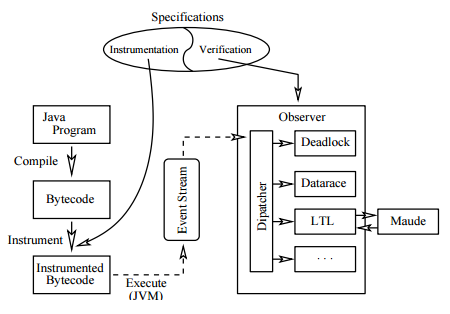
\includegraphics[width=100mm]{jpax.png}
\caption{JPaX Architecture (from \cite{havelund2001java})}
\label{img:jpax}
\end{center}
\end{figure}

JavaMaC \citep{kim2004java} is a ``run-time assurance system'' for Java programs while Mac means Monitoring and Checking. Its architecture is shown in Figure \ref{img:javamac}. Two definition languages are proposed: one for high-level specification which specifies required properties, another for low-level specification which defines the events and conditions. During the preparation, a ``filter'' and an ``event recognizer'' which are used to collect the necessary event traces are generated from the low-level specification, and a ``run-time checker'' is generated from the high-level spec. When running with the target program, events collected by the ``filter'' and ``event recognizer'' are sent to the ``run-time'' checker which is then responsible for the runtime verification work.

\begin{figure}[h]
\begin{center}
\centering
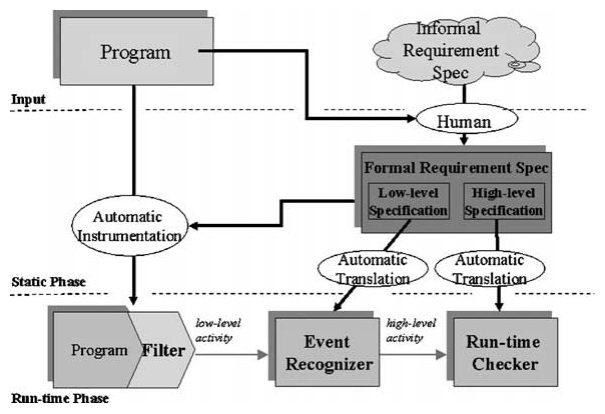
\includegraphics[width=100mm]{javamac.png}
\caption{MaC Architecture (from \cite{kim2004java})}
\label{img:javamac}
\end{center}
\end{figure}

\cite{d2005event} presents a logic named HAWK and its tools for RV of Java programs. HAWK is in fact built on EAGLE, another temporal logic which is considered more expressive \citep{barringer2004rule}. Although HAWK is event-based in contrast to state-based EAGLE, HAWK specifications are translated to EAGLE monitors. As Figure \ref{img:eagle} describes, during program execution, the EAGLE state is updated by instrumented program which then notifies the EAGLE observer. After that, the observer assesses the formul\ae{} in the current state to produce a result. 

\begin{figure}[h]
\begin{center}
\centering
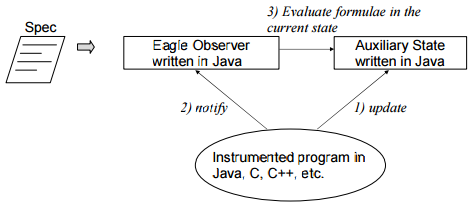
\includegraphics[width=100mm]{eagle.png}
\caption{Eagle Architecture (from \cite{d2005event})}
\label{img:eagle}
\end{center}
\end{figure}

Temporal Rover \citep{drusinsky2000temporal} is a commercial runtime verification tool based on LTL and MTL (Metric Temporal Logic). The specification code of Temporal Rover is inserted into the source code of Java, C, C++ or HDL and then converted into a compilable source file of corresponding language. A Temporal-Rover runtime verification system normally has two parts: host and target. The host is responsible for the verification while the target performs the computation of propositional formul\ae{} and sends back the results to the host via serial port, RPC or other customizable protocol.

Each of the frameworks discussed above hardwires a different specification formalism, which suggests that a general specification formalism serving all purposes does not exist. To be more expressive and generic, \cite{chen2007mop} introduced customizable and extensible ``logic-plugins'' in their runtime framework MOP and designed its architecture shown in Figure \ref{img:mop} with two layers: one is called ``language clients'' which support different programming languages, while another is ``logic repository'' which includes and manages various ``logic-plugins'' to support different specification formalisms, such as : Linear Temporal Logic (ltl), Finite State Machines (fsm), Extended Regular Expressions (ere), Context Free Grammars (cfg) and String Rewriting Systems (srs).

\begin{figure}[h]
\begin{center}
\centering
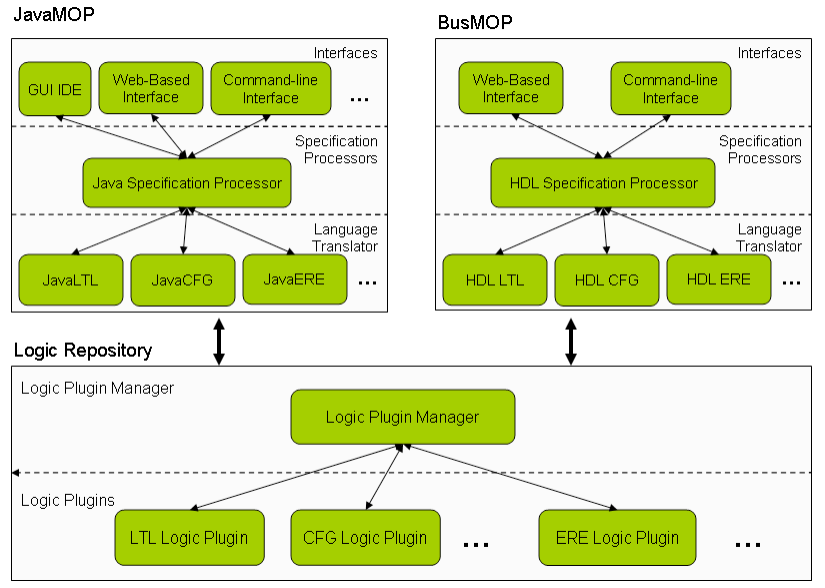
\includegraphics[width=130mm]{mop.png}
\caption{MOP Architecture (from \cite{chen2007mop})}
\label{img:mop}
\end{center}
\end{figure}

Besides the frameworks presented above, there are also lots of other frameworks invented for their corresponding requirements or specific temporal logics. Comparing these frameworks, we can find that they have their specialties as well as they share some common characters. For example, nearly all frameworks support online monitoring mode, Java programming language and network communication perhaps because these features are the most popular requirement in industry. Temporal Rover is a commercial RV framework, so it has to support more programming languages and supply more data collection options in order to expand its marketing. MOP was designed to be extremely general, resulting that most components can be changed or separately optimized.
